\documentclass[12pt]{article}
\usepackage{graphicx}
\usepackage{wrapfig}
\usepackage{amsmath}
\usepackage[brazil]{babel}
\usepackage[a4paper, left=3cm, top=3cm, right=2cm, bottom=2cm]{geometry}
\usepackage{float}
\usepackage{hyperref}
\usepackage[square,numbers]{natbib}
\setcounter{secnumdepth}{4}
\setcounter{tocdepth}{4}
\bibliographystyle{abbrvnat}


\begin{document}


\begin{titlepage}
    \begin{center}
        Universidade Federal de Santa Catarina\\
        Departamento de Engenharias da Mobilidade \\ Eletrônica Análogica - EMB5116\\

        \vspace{1.5cm}
        
\includegraphics[width=0.28\textwidth]{./images/vertical_sigla_fundo_claro.png}

        \vspace*{1.5cm}
        \fontsize{12pt}{16pt}\textbf{Eletrônica Analógica - Trabalho 2}

        \vspace*{1.5cm}
        Dr. Prof. Milton Evangelista de Oliveira Filhos

        \vspace*{1.0cm}
        \begin{tabular}{c c}
                André Stein - 22201053\\
                Danilo Machado - 22203056\\
                Pedro Lauxen - 22201064\\
        \end{tabular}

        \vspace*{\fill}
        {Joinville\\
        2025}
    \end{center}
\end{titlepage}


\tableofcontents\renewcommand*\contentsname{Sumário}
\newpage

\section{Introdução}

    Dispositivos transistores são utilizados comumente como meios de amplificar, ou chavear um circuito, de forma que o mesmo opere da maneira desejada no circuito. Dentre os transistores existentes os tipos mais comuns são os bipolares de junção,cujo são componentes formados pela junção de semicondutores,de forma que os agregando em conjuntos do tipo NPN ou PNP, forma-se um dispositivo que opera conforme é configurada sua polarização, porém assim como há a existência de componentes específicos dentro do mundo dos capacitores e resistores, dentro do mundo dos transistores existem os transistores de efeito de campo, que utilizam outra forma de controlar o fluxo de corrente por semicondutores. Neste trabalho serão descritos diferentes transistores de efeito de campo(FET) como,FET de junção (JFET),FET de Metal-Óxido-Semicondutor(MOSFET) e por último o Transistor Bipolar de Porta Isolada(IGBT) determinando como funciona cada um desses componentes, assim como será feita a comparação entre os mesmos, e por fim a comparação direta com transistores bipolares de junção.

\newpage

\section{Transistores de Efeito de Campo}

\section{FET de junção(JFET)}

\section{FET de Metal-Óxido-Semicondutor(MOSFET)}

        \begin{figure}[htpb!]

            \centering
            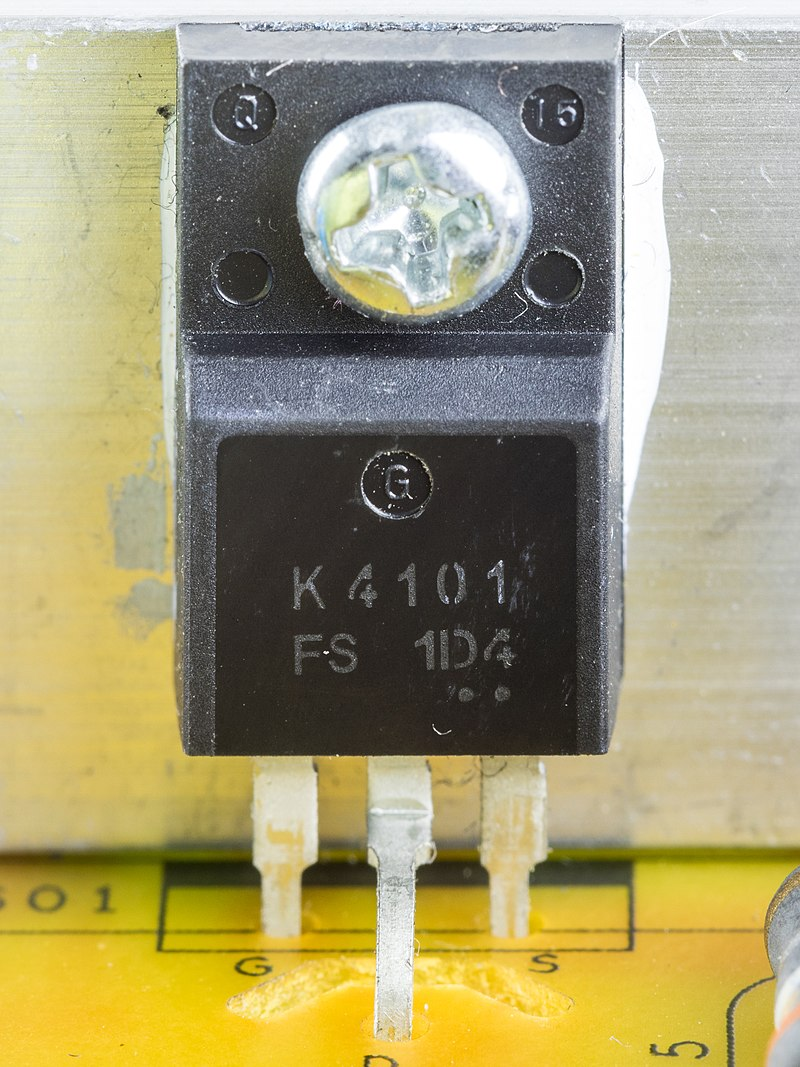
\includegraphics[width=0.2\textwidth]{./images/Dell_Professional_P2212H_-_power_supply_board_-_K4101FS-2149.jpg}
            \caption{MOSFET de potência.}

        \end{figure}

    O transistor MOSFET (acrônimo de Metal Oxide Semiconductor Field Effect Transistor, ou transistor de efeito de campo semicondutor de óxido metálico — TECMOS), é o tipo mais comum de transístores de efeito de campo em circuitos tanto digitais quanto analógicos. Seu princípio básico foi proposto pela primeira vez por Julius Edgar Lilienfeld, em 1925.

    Os transistores de efeito de campo diferentemente dos transistores bipolares comuns são típicos amplificadores de tensão e não de corrente. Enquanto a corrente de coletor de um transistor comum é função da corrente de base, num transistor de efeito de campo, a corrente de dreno é função da tensão de comporta, conforme indica a figura \ref{fig:comparacao}.

        \begin{figure}[htpb!]

            \centering
            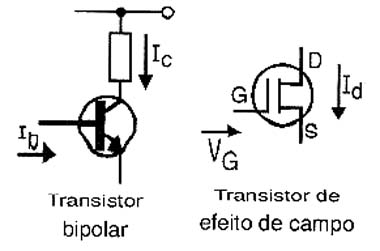
\includegraphics[width=0.4\textwidth]{./images/transisCampo.jpg}
            \caption{comparação entre transistor bipolar e transistor de efeito de campo.}
            \label{fig:comparacao}

        \end{figure}

        \begin{figure}[htpb!]

            \centering
            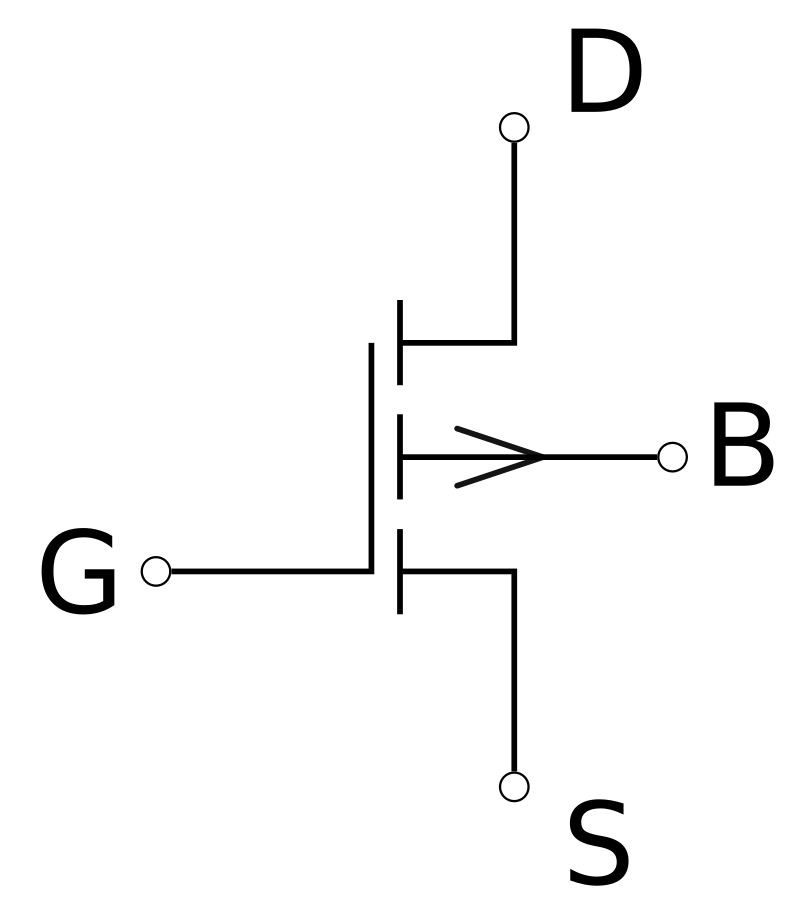
\includegraphics[width=0.2\textwidth]{./images/Mosfet-wp.svg.png}
            \caption{Símbolo de esquema elétrico de um MOSFET.}

        \end{figure}

        Uma fina película de óxido de metal isola a região de comporta da região do canal que liga o dreno à fonte. Isso faz com que a impedância de entrada do MOSFET seja muito alta, o que significa que ele consome muito pouca corrente da fonte de sinal que está dirigindo a comporta. Essa característica torna os MOSFETs ideais para circuitos de alta impedância, como amplificadores de áudio e circuitos digitais. Além disso, os MOSFETs são capazes de operar em frequências muito altas, tornando-os adequados para aplicações em rádio frequência (RF) e micro-ondas.

        \begin{figure}[htpb!]

            \centering
            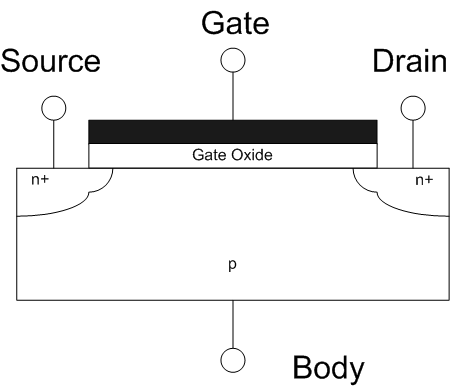
\includegraphics[width=0.3\textwidth]{./images/FET_cross_section.png}
            \caption{Símbolo de esquema elétrico de um MOSFET.}

        \end{figure}



        A palavra "metal" no nome é um anacronismo vindo dos primeiros chips, onde as comportas (gates) eram de metal. Os chips modernos usam comportas de polissilício, mas ainda são chamados de MOSFETs. Um MOSFET é composto de um canal de material semicondutor de tipo N ou de tipo P e é chamado respectivamente de NMOS ou PMOS. Geralmente o semicondutor escolhido é o silício, mas alguns fabricantes, principalmente a IBM, começaram a usar uma mistura de silício e germânio (SiGe) nos canais dos MOSFETs. Infelizmente muitos semicondutores com melhores propriedades elétricas do que o silício, tais como o arsenieto de gálio, não formam bons óxidos nas comportas e portanto não são adequados para os MOSFETs. O IGFET é um termo relacionado que significa Insulated-Gate Field Effect Transistor, e é quase sinônimo de MOSFET, embora ele possa se referir a um FET com comporta isolada por um isolante não óxido.

        O terminal de comporta é uma camada de polissilício (sílicio policristalino) colocada sobre o canal, mas separada do canal por uma fina camada de dióxido de silício isolante. Quando uma tensão é aplicada entre os terminais comporta (gate) e fonte (source), o campo elétrico gerado penetra através do óxido e cria uma espécie de "canal invertido" no canal original abaixo dele. O canal invertido é do mesmo tipo P ou tipo N, como o da fonte ou do dreno, assim, ele cria um condutor através do qual a corrente elétrica possa passar. Variando-se a tensão entre a comporta e a fonte se modula a condutividade dessa camada e torna possível se controlar o fluxo de corrente entre o dreno e a fonte. Existem também modelos de Amplificador operacional baseados na tecnologia FET/MOSFET, muito úteis e com grande utilização na indústria eletrônica.




\section{Transistor Bipolar de Porta Isolada(IGBT)}

    O tipo de transistor IGBT, pode ser definido de maneira técnica como um transistor formado com 3 terminais formando uma espécie de chave eletrônica, tendo como principal objetivo combinar alta eficiência com comutação rápida. A sua semelhança com o tiristor pode causar certa confusão pois sua definição também inclui a chave tripla,porém a ação do tiristor é diferente no sentido de, permitir apenas a ação do transistor presente, na faixa de operação do tiristor.

        \subsection{Tiristor}

        O tiristor diferente do IGBT,é um componente constituido de camadas que formam uma junção PNPN constituindo 4 camadas de formação tornando assim sua composição uma espécie de junção entre transistores do tipo PNP e NPN, seus terminais possuem ânodo,cátodo, e uma porta que funciona como um interrruptor, possuindo como modo de operação bloqueio reverso,direto e condução direta para controlar o fluxo de corrente no circuito. Suas aplicações são voltadas para sistemas de controle como controle de potência, motores e circuito de alarme.

        \begin{figure}[H]
            \centering
            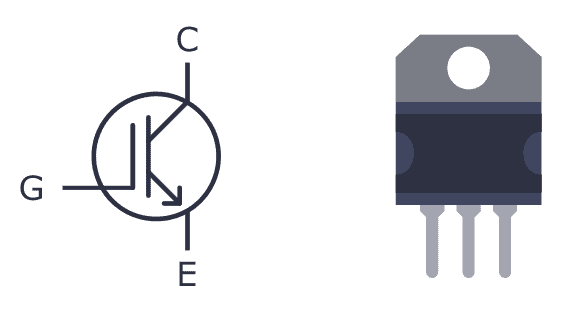
\includegraphics[width=0.45\textwidth]{./images/IGBT.png}
            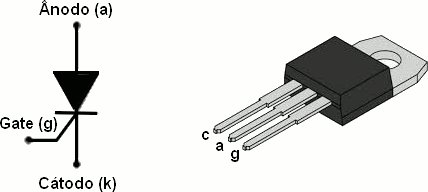
\includegraphics[width=0.45\textwidth]{./images/tiristor.png}
        \caption{À esquerda: IGBT. À direita: Tiristor.}
        \end{figure}
        \subsection{Estrutura do IGBT}

        A célula IGBT é construída semelhante ao MOSFET, porem a mudança está em que a parte n${^+}$ é substituida por uma camada coletora p${^+}$ desse modo forma um transistor PNP vertical, tal região coletora cria uma espécie de conexão do tipo Transistor Bipolar PNP com um MOSFET com a parte n${^+}$ na superfície, juntando assim o "melhor" dos dois dispositivos formando uma estrutura NPNP.

        \subsection{Modelagem matemática e física do IGBT}
        \subsection{Design do componente}
        \subsection{}
        \subsection{}

\section{Conclusões}

    Com este trabalho foi possível compreender de forma mais clara os tipos e funcionalidades dos resistores e capacitores em diferentes circuitos eletrônicos, abordando desde materiais de fabricação dos componentes a casos especiais de aplicações específicas. Com isso evidenciando que a escolha do tipo adequado de componente é parte fundamental na construção de qualquer tipo de circuito, dependendo diretamente das condições de operação do circuito, sendo necessário considerar a tolerância, dissipação de potência, tensão de trabalho, resistência interna do capacitor e estabilidade térmica necessária para cada caso.

    Dessa forma, vemos que os resistores e capacitores não devem ser vistos apenas como elementos básicos em um esquema eletrônico, mas como peças-chave que definem o desempenho, a segurança e a confiabilidade de um projeto. Sua seleção adequada exige não apenas conhecimento técnico, mas também compreensão prática das condições reais de operação.

\newpage

\bibliography{referencia}
\end{document}
